\documentclass[12pt]{beamer}
\usepackage[utf8]{inputenc}
\usepackage[main=ukrainian,english]{babel}
\usepackage{amsmath}
\usepackage{multicol}
\usetheme{Berkeley}
\logo{
\includegraphics[height=1.5cm]{images/Lviv_Polytechnic} }

\title{Алгоритми та програмне забезпечення для усунення шуму на зображеннях}
\author{Ольга Павлюк \newline \newline {керівник: к.т.н., ст. викл. Роман Кутельмах}} 
%\subtitle{{ дослідження,  розроблення алгоритмів та програмного забезпечення}}
\institute{Національний університет "Львівська політехніка", кафедра ПЗ}

\date{\today}

\begin{document}

\begin{frame}
	\titlepage
\end{frame}

\begin{frame}
	\frametitle{Зміст} 
	\tableofcontents
\end{frame}

\section{Задача усунення шуму на зображеннях}
\begin{frame}\frametitle{Задача усунення шуму на зображеннях}
	\begin{block}{Шум}
	випадкові, відсутні на реальному зображенні відхилення інтенсивності
	\end{block}
	\begin{center}
		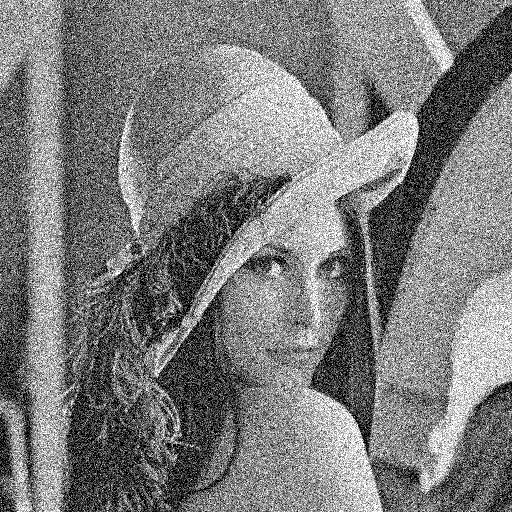
\includegraphics[scale=0.2]{images/noisy_lena}
	\end{center}
	
\end{frame}	
\begin{frame} \frametitle{Задача усунення шуму на зображеннях}
\begin{itemize}
		\item поширена проблема для цифрових зображень у багатьох галузях
		\item виникає при недостатьому освітленні та високій ISO камери
	\end{itemize}
	
	\begin{block}{Формальний опис}
		v(i) = u(i) + n(i), де i - піксель зображення \linebreak
		v(i) - спостережене значення, u(i) - справжнє значення \linebreak
		n(i) - значення шуму 
	\end{block}
\end{frame}


\begin{frame}\frametitle{Параметри оцінки алгоритмів усунення шуму}
	\begin{enumerate}
		\item автоматичні: Peak Signal-to-Noise Ratio \linebreak
		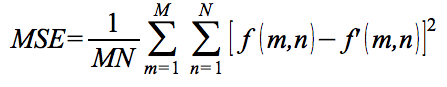
\includegraphics[scale=0.4]{images/mse} \linebreak
		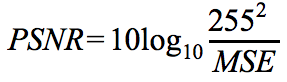
\includegraphics[scale=0.4]{images/psnr} \linebreak
		\item візуальна оцінка: вирішальний критерій вибору алгоритму
	\end{enumerate}
\end{frame}


\begin{frame}\frametitle{Існуючі методи усунення шуму}	
	\begin{multicols}{2}
		алгоритми з патчами\linebreak O(n^{2}) \linebreak
		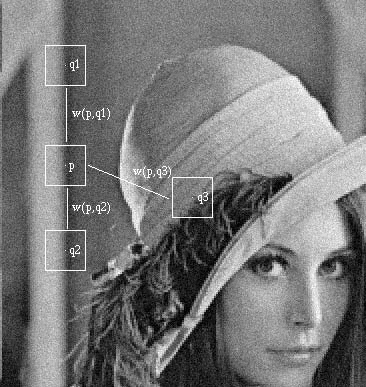
\includegraphics[scale=0.35]{images/patch}
		
		\columnbreak
		
		алгоритми з вейвлетами\linebreak O(n*\log{n}) \linebreak
		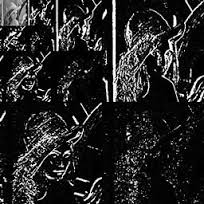
\includegraphics[scale=0.65]{images/dwt}
	\end{multicols}
	
\end{frame}

\begin{frame}\frametitle{Існуючі методи усунення шуму}	
	\begin{multicols}{2}
		алгоритми з патчами 
		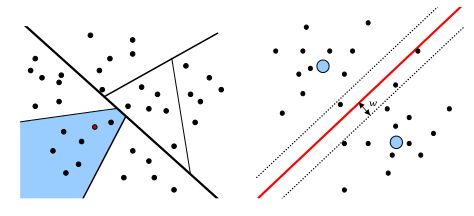
\includegraphics[scale=0.25]{images/cluster} \linebreak
		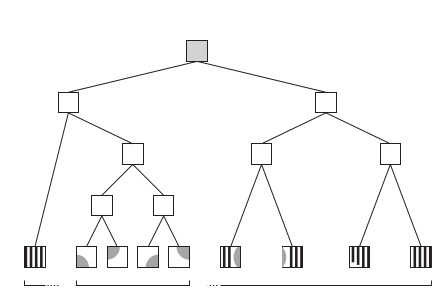
\includegraphics[scale=0.2]{images/patch2} \linebreak
		дерево кластерів: нижча складність, нижча якість
		\columnbreak
		
		алгоритми з вейвлетами
		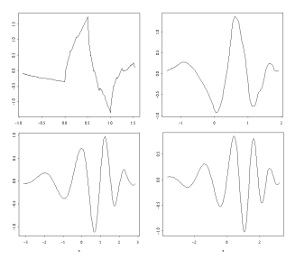
\includegraphics[scale=0.4]{images/waves} \linebreak
		базові функції вейвлета: різна роздільна здатність
	\end{multicols}
\end{frame}

\begin{frame}\frametitle{Вейвлет-алгоритми}
	\begin{enumerate}
		\item виконується рекурсивна декомпозиція сигналу до заданого рівня\linebreak
		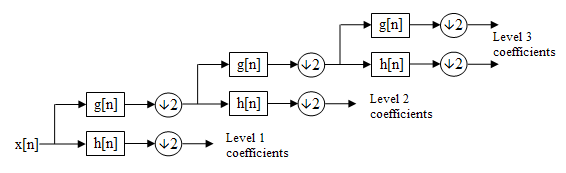
\includegraphics[scale=0.3]{images/filter_bank} \linebreak
		\item коефіцієнти аналізуються "знизу вверх" 
		\item застосовується порогове відсікання: \linebreak
		\[
		w(x)= 
		\begin{cases}
		w(x),& \text{if } \mid{w(x)}\mid \geq threshold\\
		0,              & \text{otherwise}
		\end{cases}
		\]
		\item до отриманих коефіцієнтів застосовується зворотнє перетворення
	\end{enumerate}
\end{frame}

\section{Завдання магістерського дослідження}
\begin{frame}\frametitle{Завдання магістерського дослідження}
	\begin{block}{Об'єкт}
		процес усунення шуму на зображеннях
	\end{block}
	\begin{block}{Предмет}
		методи, алгоритми та програмне забезпечення для усунення шуму на зображеннях
	\end{block}
	\begin{block}{Мета}
		розроблення алгоритмів та програмного забезпечення для усунення шуму на зображеннях
	\end{block}
\end{frame}

\section{Розроблений алгоритм}
\begin{frame}\frametitle{Розроблений алгоритм}
	\begin{itemize}
		\item є модифікацією Ridgelet-перетворення
		\item розроблений для роботи на GPU (GLSL)
	\end{itemize}
\end{frame}
\begin{frame}\frametitle{Ridgelet-перетворення }
	\begin{center}
	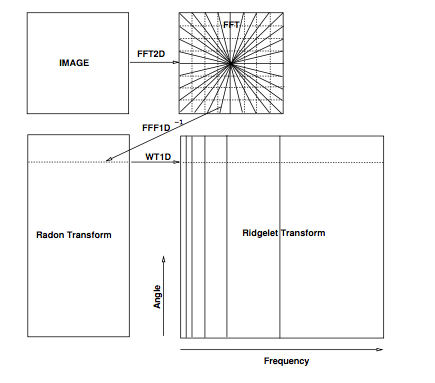
\includegraphics[width=0.65\textwidth]{images/ridgelet}
	\end{center}
	\linebreak Це вейвлет-перетворення, застосоване до ліній у просторі Радона
		 
\end{frame}
\begin{frame}\frametitle{Перетворення Фур'є}
	\begin{itemize}
		\item базовий метод для всіх алгоритмів, що працюють з частотами   
		\item сигнал можна представити у вигляді суми синусоїд з різними амплітудами та зсувом
		\item операція згортки сигналу з фільтром довільної довжини виконується за лінійний час
	\end{itemize}
	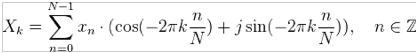
\includegraphics[scale=0.5]{images/fourier_1d} 
\end{frame}
\begin{frame}\frametitle{Перетворення Радона (Radon Transform) }
	це інтегральне перетворення, яке для кожної прямої на зображенні ставить їй у відповідність суму пікселів зображення на цій прямій\linebreak
	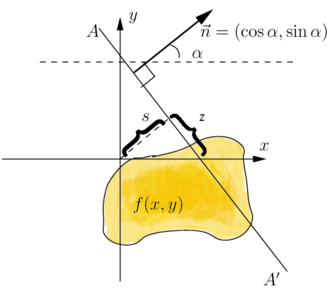
\includegraphics[scale=0.4]{images/radon} \texttt{\char32}
	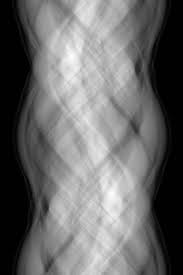
\includegraphics[scale=0.4]{images/sinogram} 
\end{frame}
\begin{frame}\frametitle{ Візуалізація перетворення Радона }
	\begin{multicols}{2}
		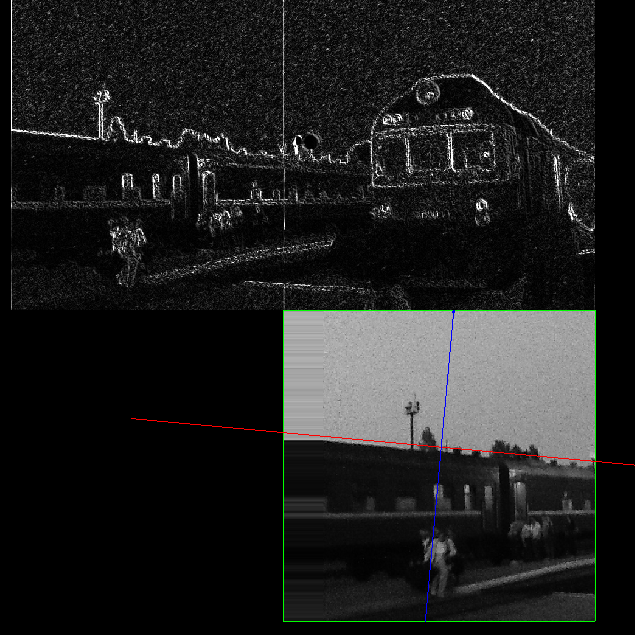
\includegraphics[scale=0.19]{images/radon_fa} 
		\columnbreak	
		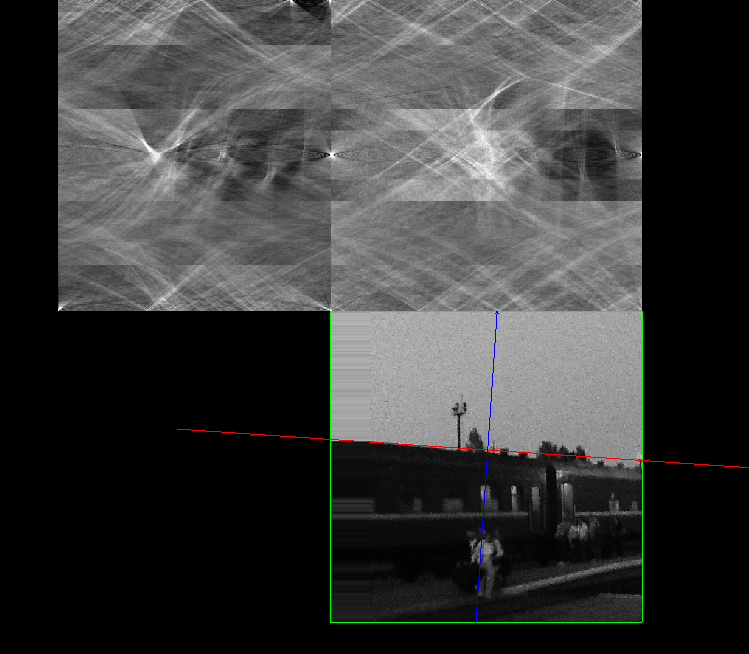
\includegraphics[scale=0.185]{images/radon_fa_2}
	\end{multicols}
	
\end{frame}
\begin{frame}\frametitle{Projection-Slice Theorem }
	Зв'язок між перетворенням Фур'є та перетворенням Радона \linebreak
	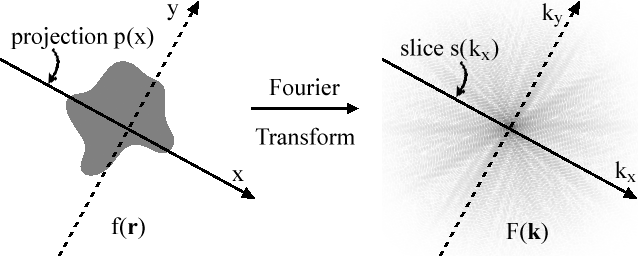
\includegraphics[scale=0.4]{images/projection_slice} 
\end{frame}

\begin{frame}\frametitle{Ректополярна решітка}
	\begin{center}
	\begin{wrapfigure}
		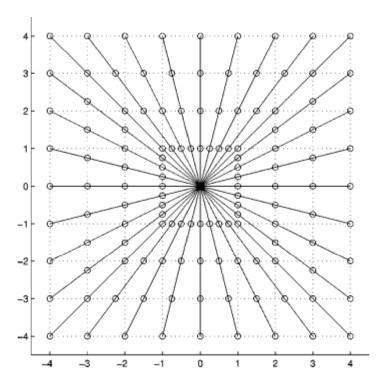
\includegraphics[width=0.5\textwidth]{images/rp_grid}
	\end{wrapfigure}
	\end{center}
	\linebreak Розглядаються {2n} прямих, які проходять через центр зображення FFT
	\linebreak Використовується інтерполяція методом найближчого сусіда
\end{frame}
\begin{frame}\frametitle{Зворотнє перетворення Радона}
	Використовується білінійна інтерполяція  \linebreak
	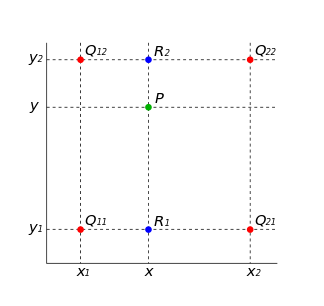
\includegraphics[scale=0.35]{images/bilinear} \linebreak
{P = ax + by + cxy + d} \newline
{ax_{1} + by_{1} + cx_{1}y_{1}+d = Q_{11}} \newline
{ax_{1} + by_{2} + cx_{1}y_{2}+d = Q_{21}} \newline
{ax_{2} + by_{1} + cx_{1}y_{1}+d = Q_{12}} \newline
{ax_{2} + by_{2} + cx_{2}y_{2}+d = Q_{22}} \newline
\end{frame}

\begin{frame}\frametitle{Усунення шуму в просторі Радона}
	Застосовано вейвлет Добеші D4 = [0.482962, 0.836516, 0.224143, -0.129409], висока та низька частота обчислюються за формулами: \linebreak 
	v_{high}=y[2v]*D_{4}[0]+y[2v+1]*D_{4}[1]+y[2v+2]*D_{4}[2]+y[2v+3]*D_{4}[3] \linebreak \linebreak
	v_{low}=y[2v]*D_{4}[3]-y[2v+1]*D{4}[2]+y[2v+2]*D{4}[1]-y[2v+3]*D{4}[0] \linebreak
%	Вейвлет-коефіцієнти з абсолютним значенням меншим за заданий поріг σ встановлюються в 0, потім застосовується обернене перетворення.
\end{frame}

\section{Використані технології}
\begin{frame}\frametitle{Використані технології: C++ та OpenGL}
	Переваги:
	\begin{enumerate}
		\item C++: швидкість обчислень  + гнучка архітектура
		\item GLSL: обчислення на GPU в десятки разів швидше  
	\end{enumerate}
	Недоліки:
	\begin{enumerate}
		\item GLSL: труднощі при відлагодженні програм
	\end{enumerate}
	
	Приклад коду шейдера:
	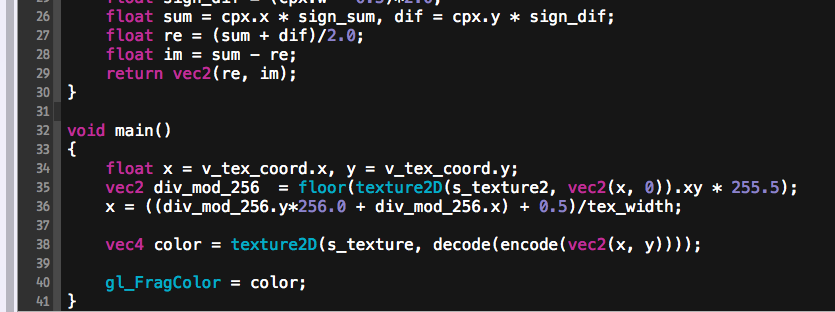
\includegraphics[height=2.5cm]{images/shader_snapshot}
\end{frame}

\section{Дослідження розробленого алгоритму}


\begin{frame}\frametitle{ Порівняння з NLM(час роботи)}
	\begin{itemize}
		\item NLM працює довго на зображеннях розміру > 1МП
		\item розроблений алгоритм працює в режимі реального часу
	\end{itemize}
	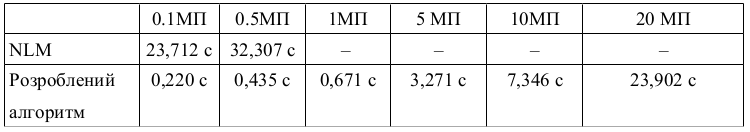
\includegraphics[scale=0.4]{images/table_imsize}
\end{frame}

\begin{frame}\frametitle{ Швидкість роботи алгоритму }
	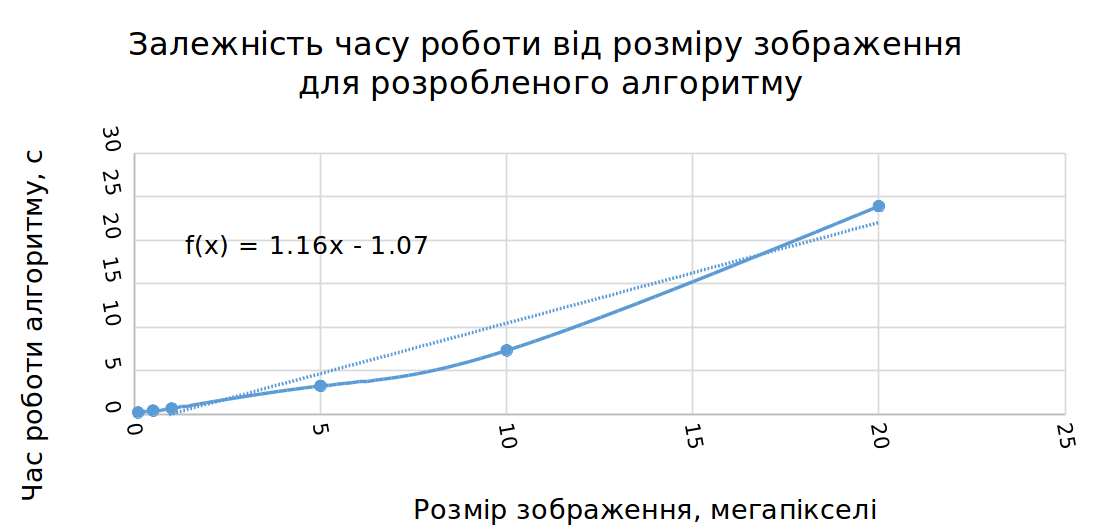
\includegraphics[scale=0.25]{images/super_graph}
\end{frame}

\section{Результати}
\begin{frame}\frametitle{ Результати }
стаття \newline {\bf «Investigation of Existing Image Denoising Algorithms»}\newline \newline   (автори — О. Павлюк та Р. Кутельмах) \newline \newline  
у Віснику НУЛП 	
\end{frame}
\begin{frame}\frametitle{ Результати}
	приклад зашумленого зображення
	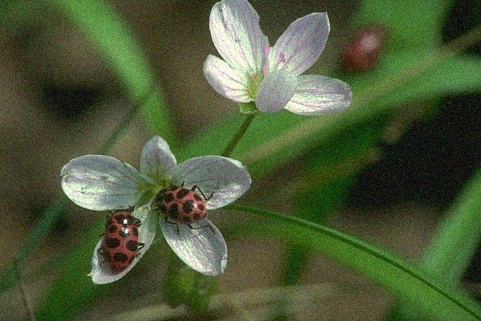
\includegraphics[scale=0.5]{images/noisy_1}
\end{frame}
\begin{frame}\frametitle{ Результати}
	результат роботи розробленого алгоритму
	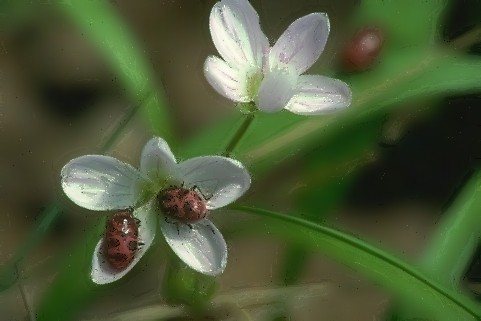
\includegraphics[scale=0.5]{images/my_1}
\end{frame}
\begin{frame}\frametitle{ Результати}
	приклад зашумленого зображення
	\includegraphics[scale=0.1]{images/al_1}
\end{frame}
\begin{frame}\frametitle{ Результати}
	результат роботи розробленого алгоритму
	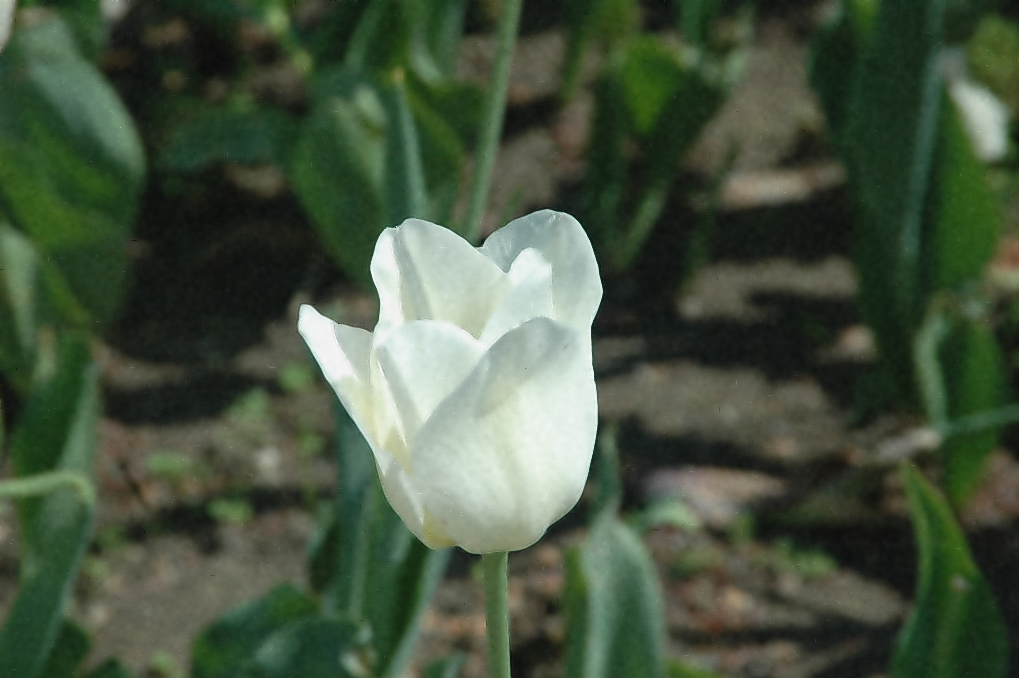
\includegraphics[scale=0.28]{images/mine_1}
\end{frame}
\begin{frame}\frametitle{ Результати}
	приклад зашумленого зображення
	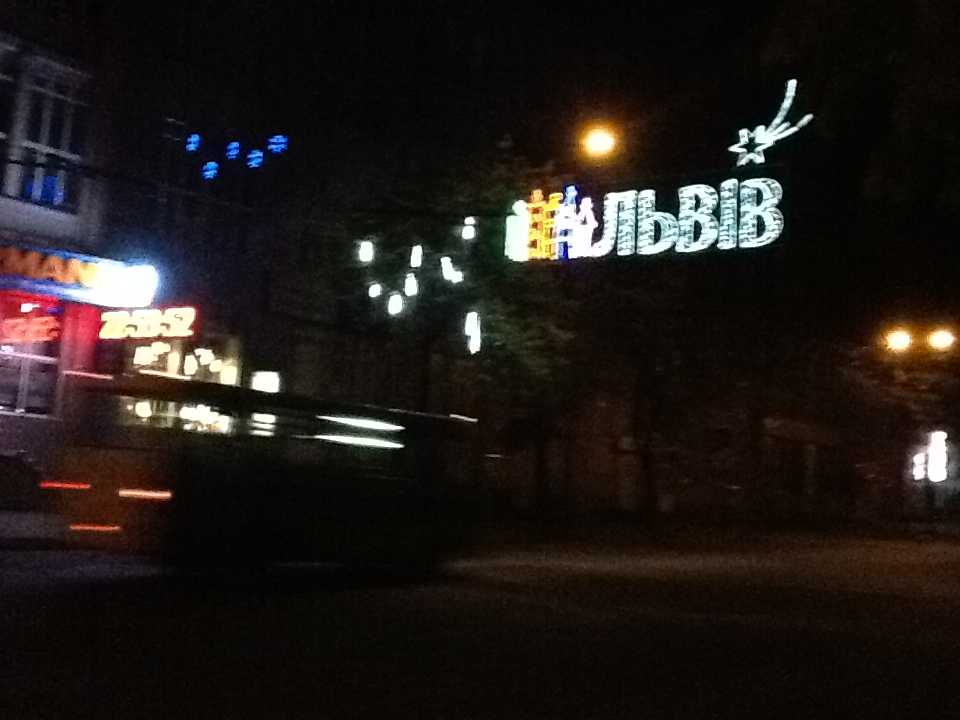
\includegraphics[scale=0.3]{images/lviv_orig}
\end{frame}
\begin{frame}\frametitle{ Результати}
	приклад роботи алгоритму Curvelab
	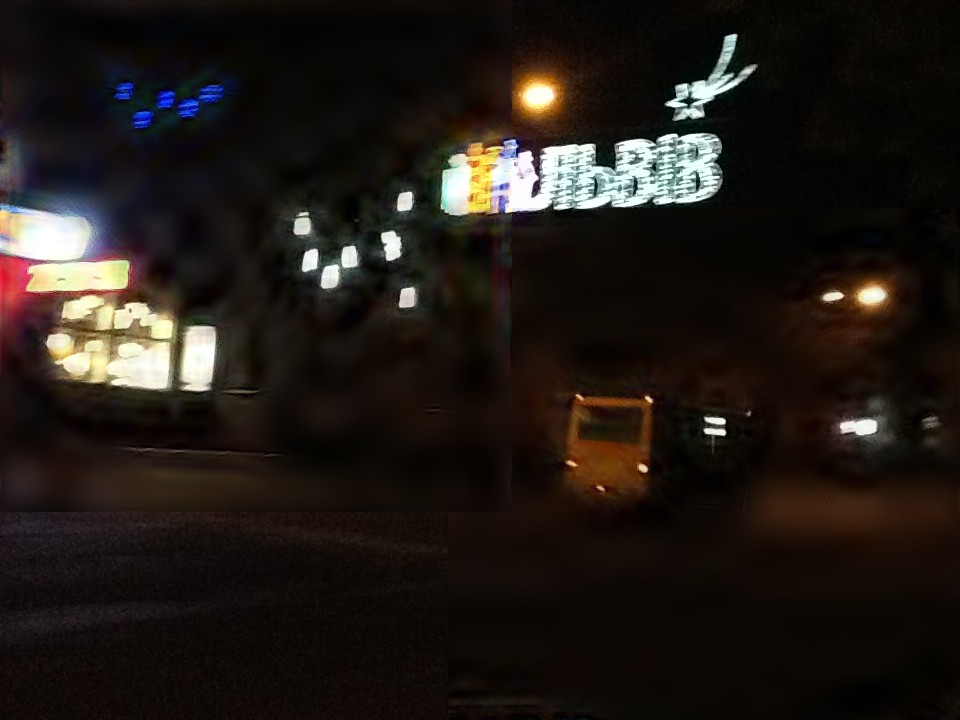
\includegraphics[scale=0.3]{images/lviv_curvelet}
\end{frame}
\begin{frame}\frametitle{ Результати}
	приклад роботи NLM
	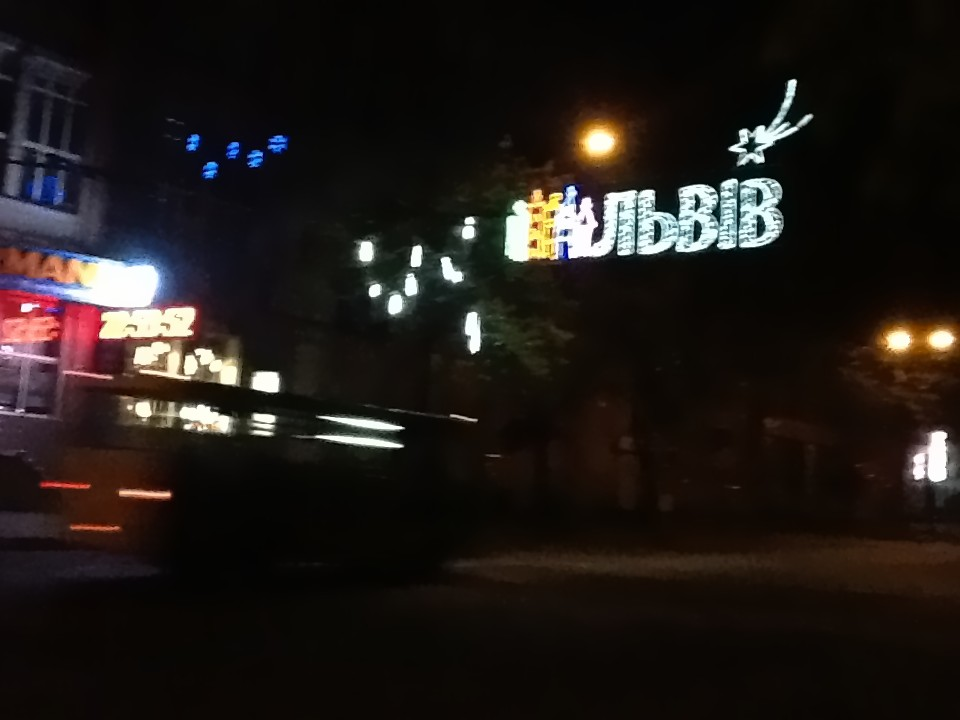
\includegraphics[scale=0.3]{images/lviv_nlm}
\end{frame}
\begin{frame}\frametitle{ Результати}
	приклад роботи розробленого алгоритму
	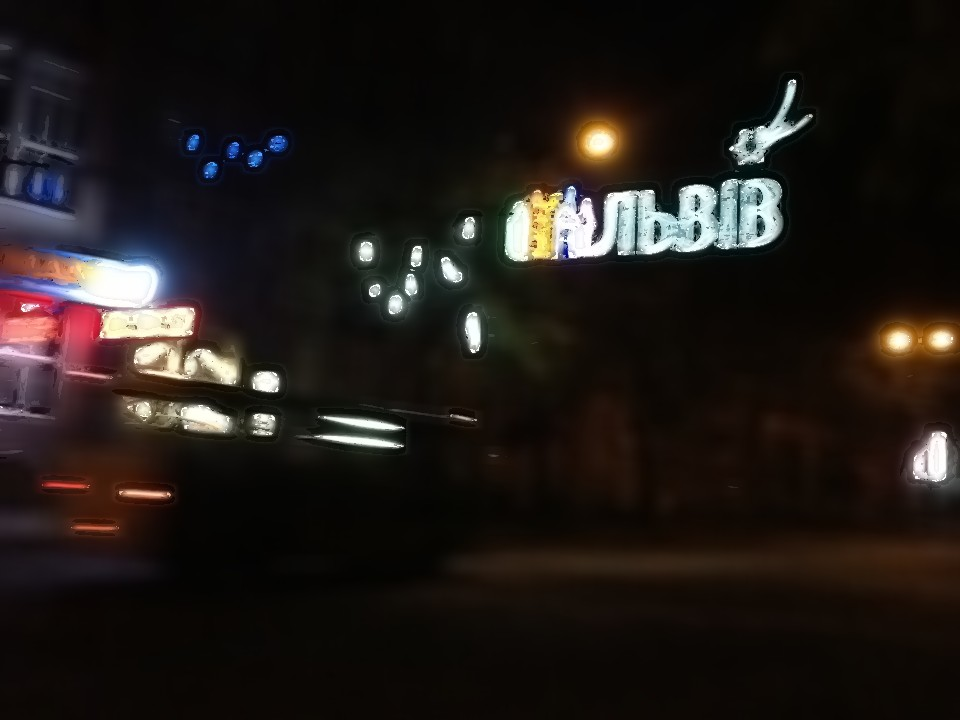
\includegraphics[scale=0.3]{images/lviv_mine}
\end{frame}
\begin{frame}\frametitle{ Результати}
	\includegraphics[scale=0.07]{images/android_rocks}
\end{frame}
\begin{frame}\frametitle{ Приклад роботи програми}
	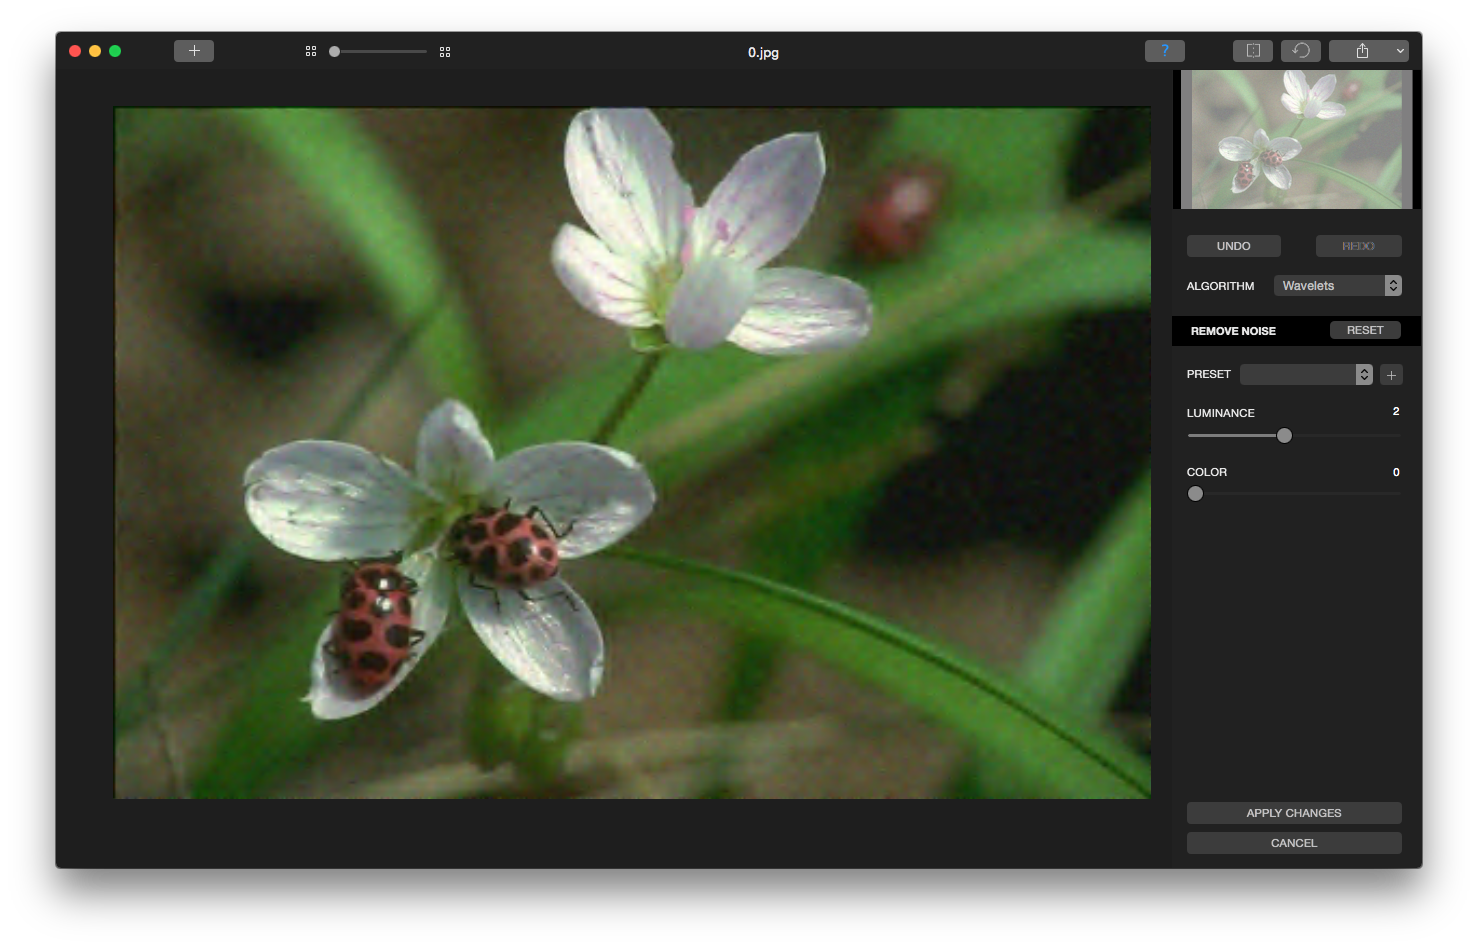
\includegraphics[scale=0.18]{images/cocoa}
	
	
\end{frame}
\begin{frame}\frametitle{ Приклад роботи програми}
	
	\includegraphics[scale=0.07]{images/android_rocks}
\end{frame}
\section{Висновки}
\begin{frame}\frametitle{Висновки }
 \begin{itemize}		
 	\item Запропоновано новий алгоритм усунення шуму на зображеннях, який базується на існуючому алгоритмі Ridgelet-перетворення
 	\item Розроблено спеціалізовану версію алгоритму для виконання на графічному процесорі
 	\item Обчислювальна складність алгоритму становить O(n*log(n)), що дає змогу застосовувати його для опрацювання зображень великого розміру (20 МП і більше)
 \end{itemize}
\end{frame}

\begin{frame}\frametitle{}
	\begin{center}
	{\Large Дякую за увагу!}
	\end{center}
\end{frame}


\end{document}
